\documentclass{article}
\usepackage{graphicx} % Nécessaire pour insérer des images
\usepackage{float}    % Pour forcer la position des figures
\usepackage{framed}   % Pour ajouter des cadres autour des images
\usepackage{listings} % Pour les exemples de code Java
\usepackage{hyperref}

\title{Couche Persistance}

\lstset{ 
    language=Java,
    frame=single,
    basicstyle=\ttfamily,
    numbers=left,
    numberstyle=\tiny,
    breaklines=true,
    showstringspaces=false,
    captionpos=b,
    xleftmargin=\parindent,
    framexleftmargin=10pt,
    framexrightmargin=10pt,
    framextopmargin=5pt,
    framexbottommargin=5pt
}

\begin{document}

\maketitle

\section{Introduction}
La couche \textbf{ persistance} agit comme un intermédiaire entre la logique métier de l'application et les systèmes de stockage des données. Ses principaux rôles incluent :
\begin{itemize}
    
    \item \textbf{Stockage des données} : Elle sauvegarde les données générées par l'application afin qu'elles puissent être récupérées plus tard, même après la fermeture de l'application.

    \item \textbf{Récupération des données} : Elle extrait les données stockées lorsque cela est nécessaire, permettant à l'application d'afficher ou de manipuler ces informations.
    
\end{itemize}

\begin{figure}[H]
    \centering
    \begin{framed}
        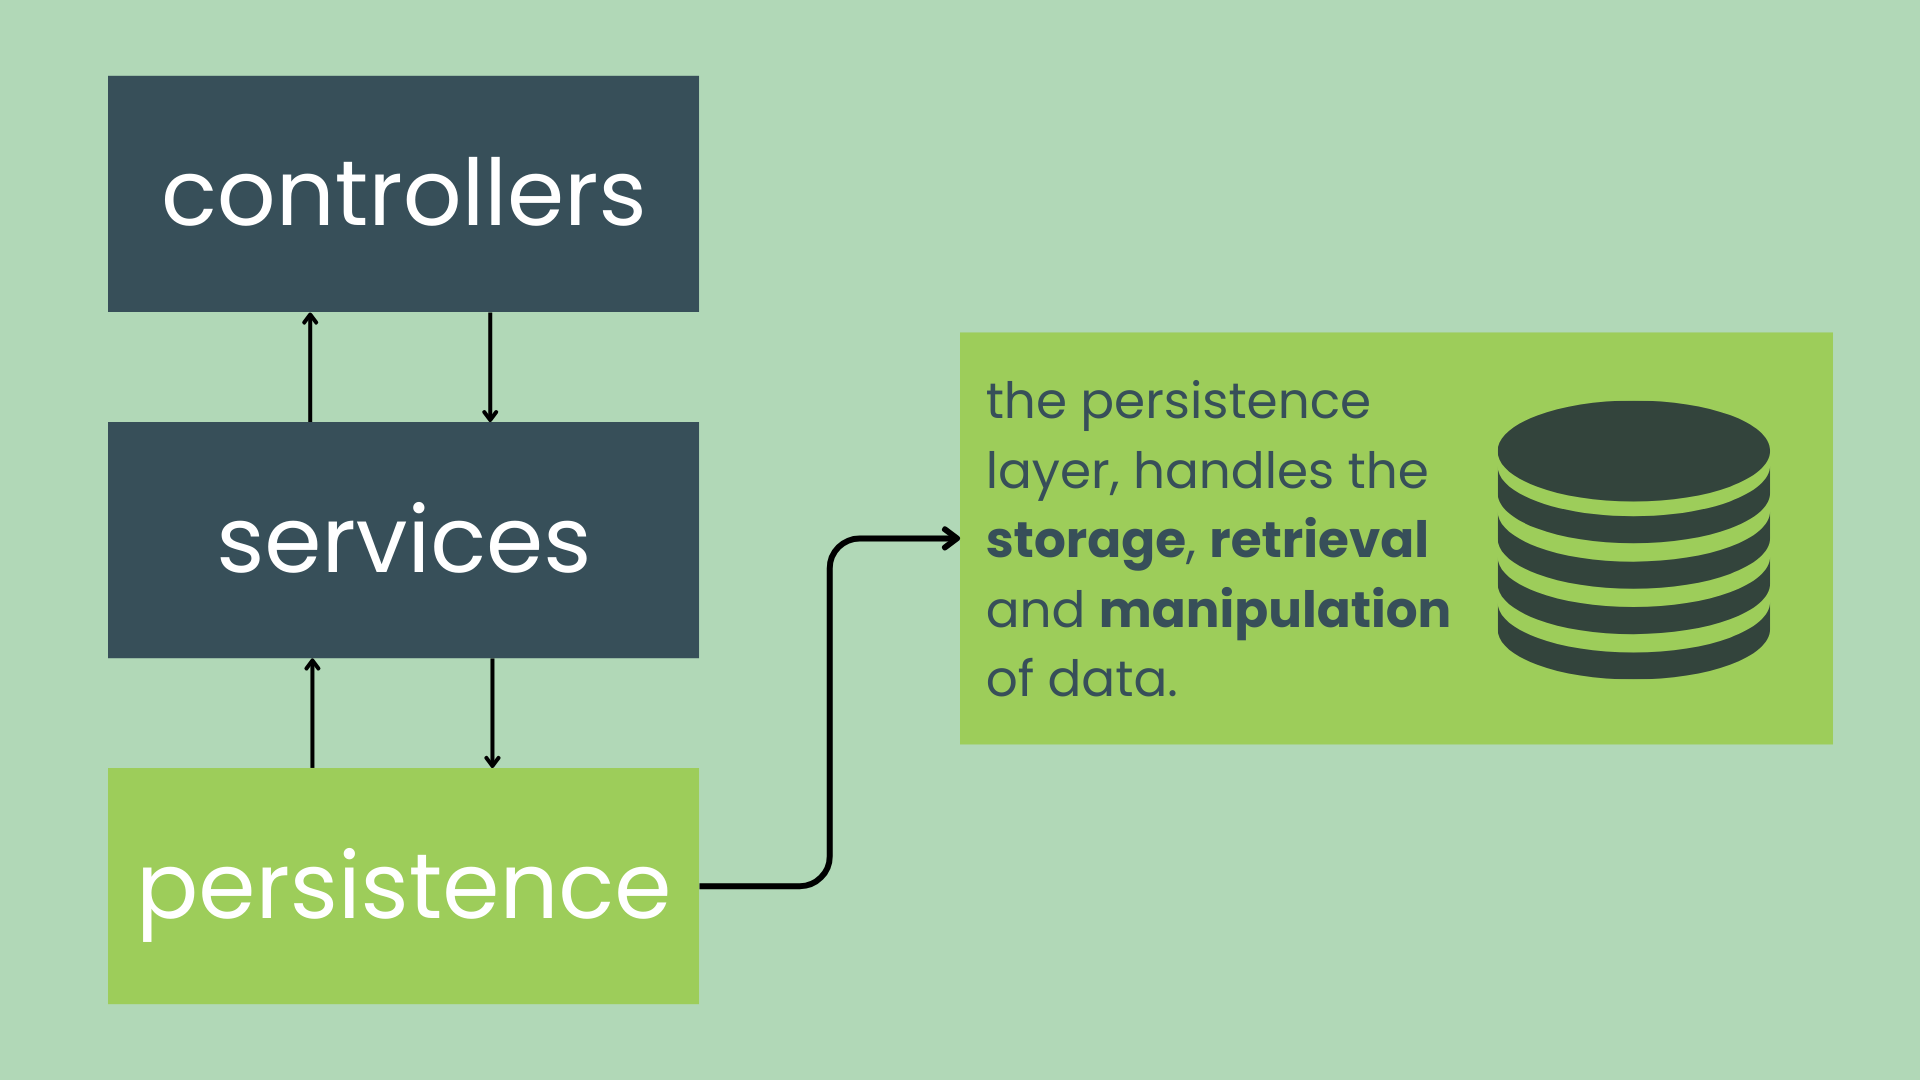
\includegraphics[width=0.8\linewidth]{images/persistence.png}
    \end{framed}
    \caption{Couches de l'application}
    \label{fig:spring-logo}
\end{figure}

Dans les sections suivantes, nous allons explorer les différentes approches pour configurer la couche de persistance dans une application multi-couches.


\section{Approche classique avec JDBC}

\subsubsection{API JDBC}

\begin{itemize}
    \item \textbf{JDBC} (Java Database Connectivity) est une API (Interface de Programmation d'Applications) qui permet aux applications Java d'interagir avec des \textbf{bases de données relationnelles}. Elle fournit un ensemble standard d'interfaces et de classes pour se connecter aux bases de données, exécuter des requêtes SQL et gérer les résultats.

    \item \textbf{API de bas niveau} : JDBC est une API de bas niveau, ce qui signifie que les développeurs doivent gérer manuellement les connexions à la base de données, traiter les exceptions SQL et fermer les ressources.
\end{itemize}

\begin{figure}[H]
    \centering
    \begin{framed}
        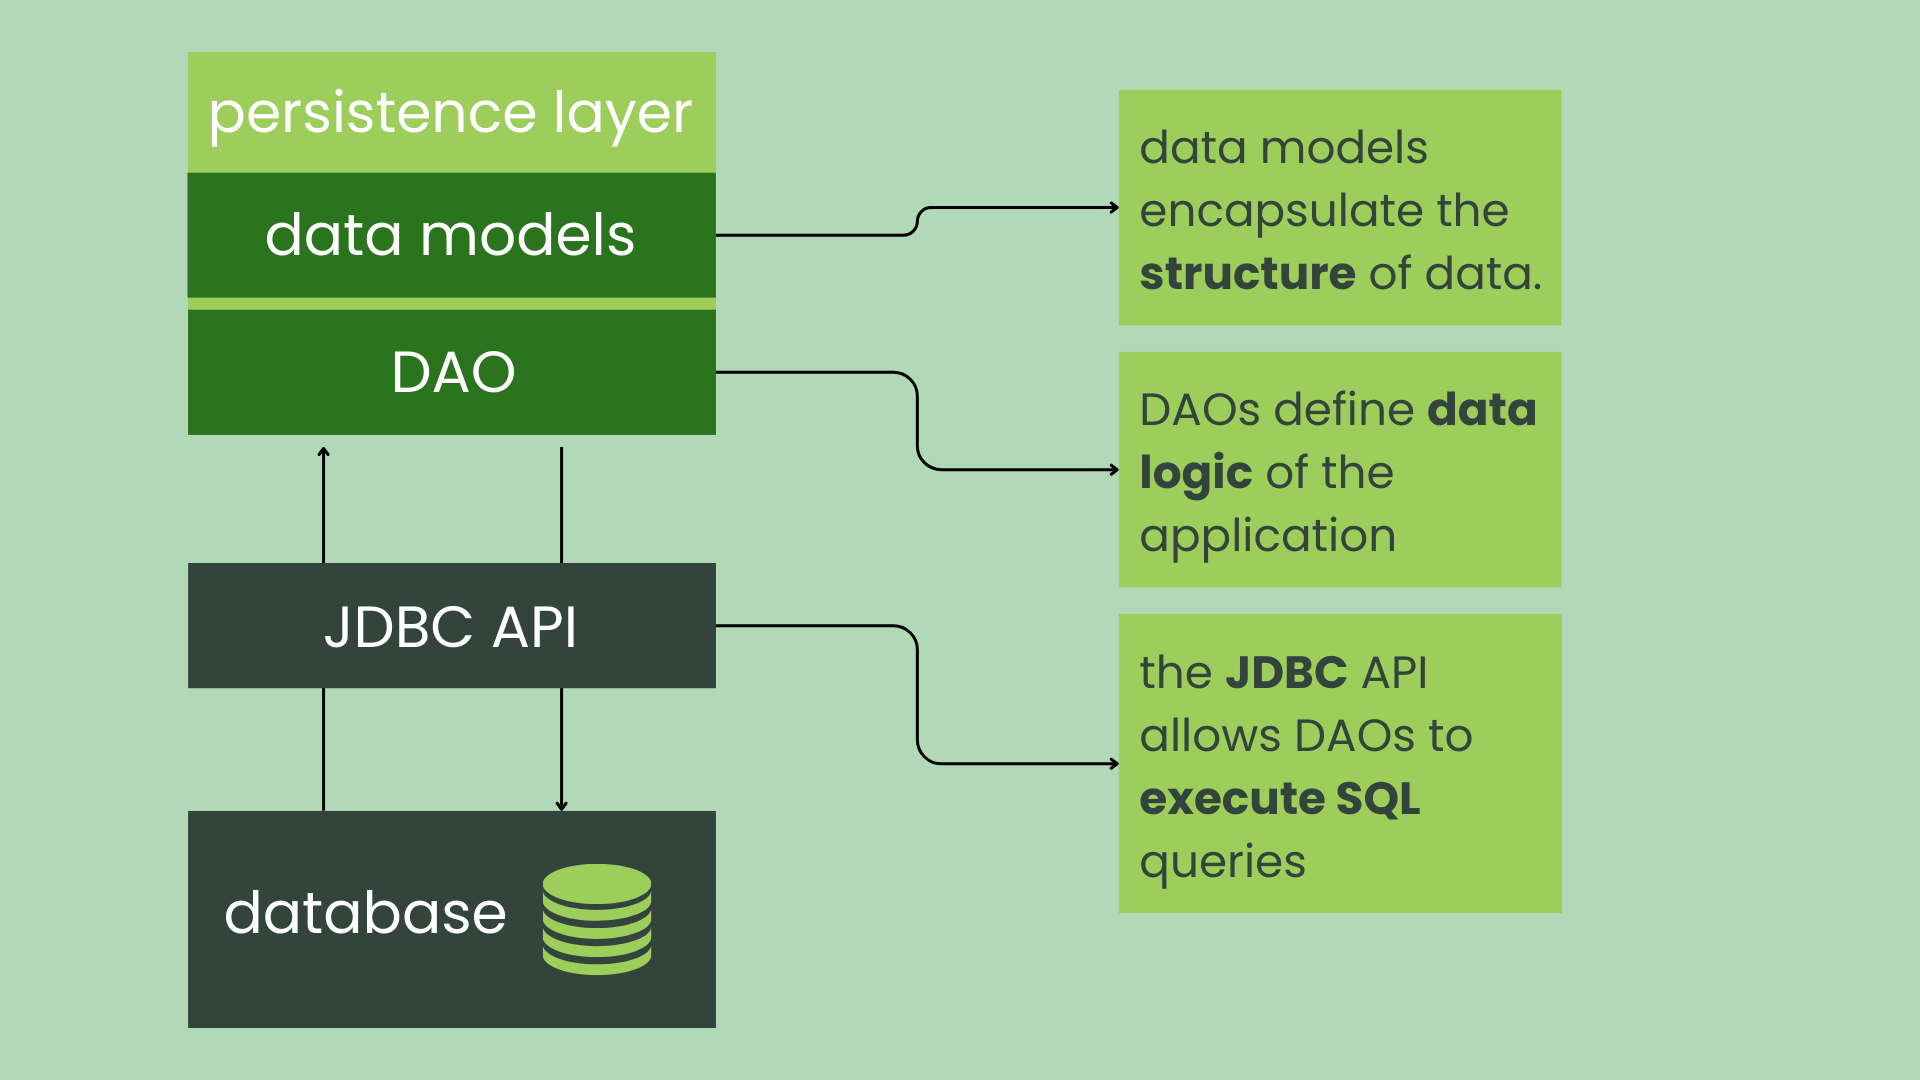
\includegraphics[width=0.8\linewidth]{images/persistence_jdbc.png}
    \end{framed}
    \caption{API JDBC}
    \label{fig:spring-logo}
\end{figure}

\subsection{Configuration de la connexion}

La première étape pour configurer la couche de persistance est d'inclure la dépendance JDBC dans le classpath de l'application, soit manuellement, soit en ajoutant la balise de dépendance appropriée dans Maven. 

L'architecture décrite ci-dessous représente la base pour établir une connexion dans l'application.

\begin{figure}[H]
    \centering
    \begin{framed}
        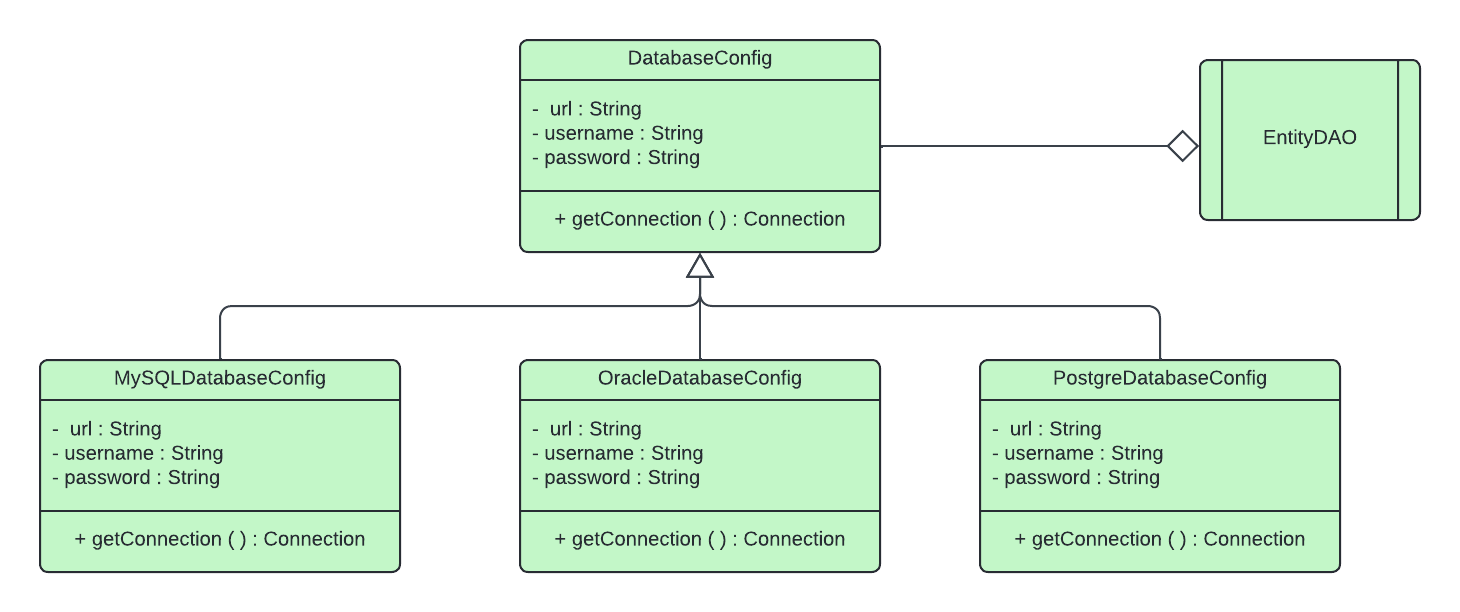
\includegraphics[width=0.8\linewidth]{images/jdbc_setup.png}
    \end{framed}
    \caption{Configuration de la connexion à la base de données}
    \label{fig:spring-logo}
\end{figure}


\begin{itemize}
    \item \textbf{Configuration de la base de données} : Cette classe abstraite définit le comportement commun pour toutes les classes de configuration de base de données. La méthode \texttt{getConnection()} de cette classe retourne la connexion à un SGBDR (Système de Gestion de Base de Données Relationnelle) spécifié.
    
    \item \textbf{Classes enfants} : Chaque classe enfant est responsable de l'établissement d'une connexion à un SGBDR spécifique, en héritant de la classe de base \texttt{DatabaseConfiguration}.
    
    \item \textbf{Classe DAO} : La classe DAO (Data Access Object) gère l'implémentation de la logique de données, exécute les requêtes SQL et utilise la connexion fournie par la classe de configuration de la base de données pour interagir avec cette dernière.
\end{itemize}

\\

\subsection{Logique métier des données}

La logique métier des données repose sur deux composants principaux. 

L'architecture ci-dessous décrit la structure générale de la couche de persistance dans une application \textbf{CRUD}.

\begin{figure}[H]
    \centering
    \begin{framed}
        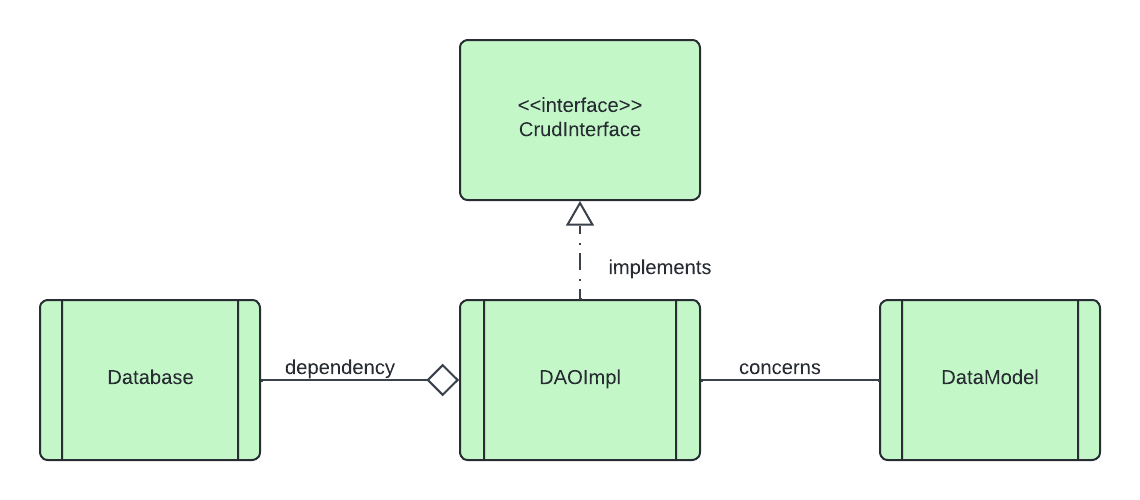
\includegraphics[width=0.8\linewidth]{images/jdbc_business_logic.png}
    \end{framed}
    \caption{Architecture de la couche de persistance dans une application CRUD}
    \label{fig:spring-logo}
\end{figure}
\subsubsection*{Composants clés :}

\begin{itemize}
    \item \textbf{Modèle de données} : Une classe qui définit le comportement commun pour toutes les classes concrètes de modèle de données, représentant la structure des données gérées par l'application.

    \item \textbf{Interface CRUD} : Une interface qui définit les signatures des méthodes pour les opérations \textbf{\texttt{CRUD}} principales : Créer, Lire, Mettre à jour et Supprimer.

    \item \textbf{Implémentation DAO} : Classes concrètes qui implémentent les méthodes CRUD pour un modèle de données spécifique, en gérant la logique d'interaction avec la base de données.
\end{itemize}

\subsection{Exemple de code }

Voici un exemple simple illustrant comment implémenter la couche de persistance pour une entité \texttt{User} en utilisant JDBC. Cela inclut la configuration de la base de données, un modèle de données, une interface CRUD et une implémentation DAO. Le code complet est disponible sur le dépôt GitHub du projet :\\ \url{https://github.com/D0esN0tM1tter/spring_boot_project-/tree/master/supporting_project/persistence_examples/jdbc_classic_approach}.

\subsubsection{Configuration de la base de données}

La classe \textbf{DatabaseConfiguration} est une classe utilitaire abstraite qui centralise la logique de connexion à la base de données. Cela garantit que les détails de connexion (comme l'URL, le nom d'utilisateur et le mot de passe) sont gérés en un seul endroit, favorisant la réutilisabilité et la maintenabilité.

\textbf{Explication :}
\begin{itemize}
    \item \texttt{DriverManager.getConnection} : Établit une connexion à la base de données en utilisant l'URL, le nom d'utilisateur et le mot de passe spécifiés.
    \item Les constantes comme \texttt{URL}, \texttt{USER} et \texttt{PASSWORD} stockent les détails de configuration de manière sécurisée et les rendent facilement modifiables.
    \item \texttt{Connection} : Représente une connexion active à la base de données, nécessaire pour exécuter des requêtes SQL.
\end{itemize}

\subsubsection{Modèle User}

La classe \textbf{User} sert de modèle de données pour représenter la structure d'un enregistrement dans la base de données. Chaque instance correspond à une ligne de la table \texttt{users}.

\textbf{Explication :}
\begin{itemize}
    \item Les champs comme \texttt{id}, \texttt{name} et \texttt{email} correspondent directement aux colonnes de la table de la base de données.
    \item Les méthodes getter et setter permettent l'encapsulation, offrant un accès contrôlé à ces champs.
\end{itemize}

\subsubsection{Interface CRUD}

L'interface \textbf{UserDAO} définit le contrat pour effectuer des opérations \textbf{CRUD} sur les données \texttt{User}.

\textbf{Explication :}
\begin{itemize}
    \item \texttt{createUser(User user)} : Ajoute un nouvel enregistrement utilisateur à la base de données.
    \item \texttt{getUserById(int id)} : Récupère un enregistrement utilisateur basé sur son ID.
    \item \texttt{getAllUsers()} : Récupère tous les enregistrements utilisateurs de la base de données.
    \item \texttt{updateUser(User user)} : Met à jour un enregistrement utilisateur existant avec de nouvelles informations.
    \item \texttt{deleteUser(int id)} : Supprime un enregistrement utilisateur basé sur son ID.
\end{itemize}

\subsubsection{Implémentation DAO}

La classe \textbf{UserDAOImpl} implémente l'interface \texttt{UserDAO}. Elle fournit la logique concrète pour interagir avec la base de données.

\textbf{Explication :}
\begin{itemize}
    \item \texttt{PreparedStatement} : Utilisé pour exécuter des requêtes paramétrées de manière sécurisée, empêchant les attaques par injection SQL.
    \item \texttt{ResultSet} : Stocke le résultat des requêtes \texttt{SELECT}, permettant une itération sur les lignes retournées.
    \item Chaque méthode utilise un bloc \texttt{try-with-resources} pour s'assurer que les connexions, instructions et autres ressources sont automatiquement fermées.
\end{itemize}
\section{Approche JDBC template}

\subsection{JDBC template} 
Le \textbf{JdbcTemplate} de Spring est une API de haut niveau dans le framework Spring qui simplifie les interactions avec la base de données en gérant les tâches courantes telles que la gestion des connexions, l'exécution des instructions SQL et la gestion des exceptions. Cela permet de rendre le code d'accès aux données plus concis et de réduire le code répétitif associé à l'API standard \textbf{JDBC}.
\\
\textbf{REMARQUE : Pour utiliser le JDBC template, il est nécessaire de le déclarer comme dépendance dans le fichier \texttt{pom.xml}}.

\begin{figure}[H]
    \centering
    \begin{framed}
        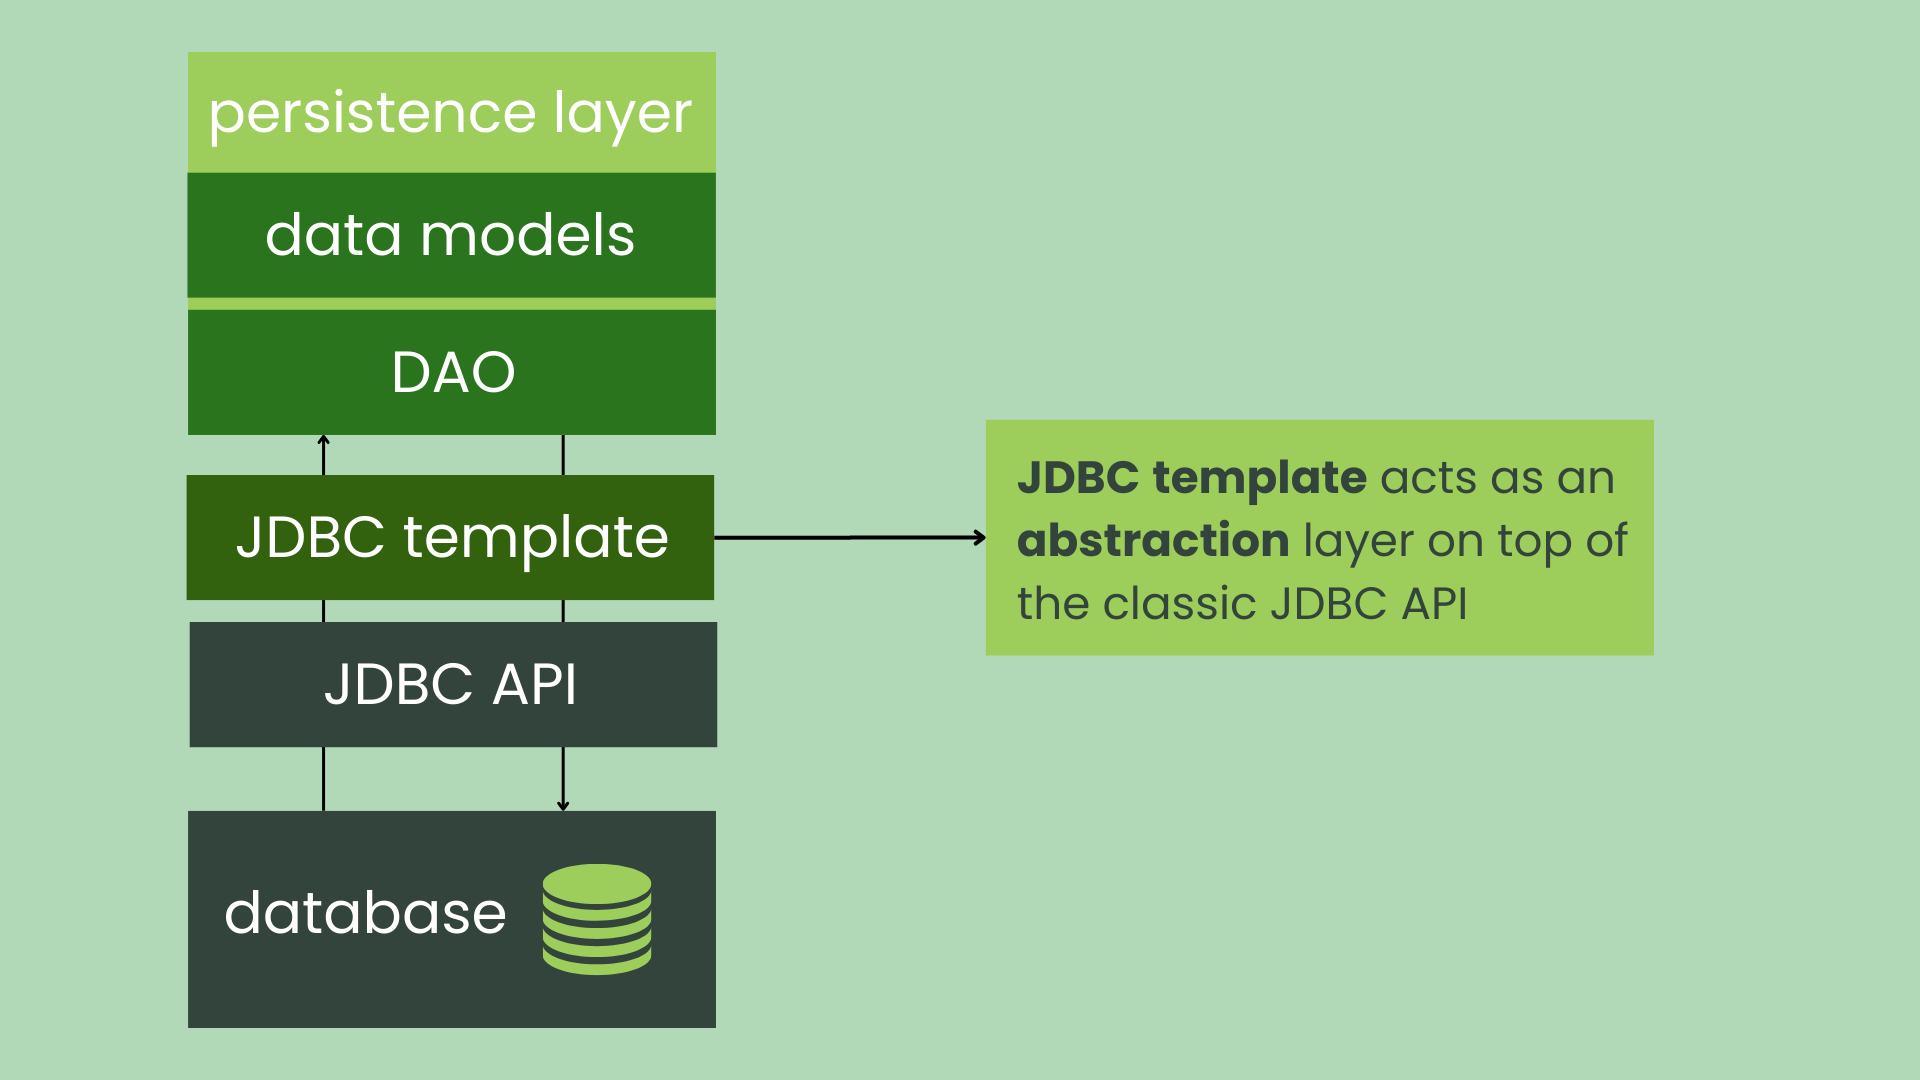
\includegraphics[width=0.8\linewidth]{images/jdbc_template.png}
    \end{framed}
    \caption{JDBC template}
    \label{fig:spring-logo}
\end{figure}

\subsection{Configuration de la connexion} 
Dans une application Spring Boot, les détails de la connexion sont définis dans le fichier \textbf{\texttt{application.properties}}. Sur la base de cette configuration, le conteneur IoC (Inversion de Contrôle) de Spring génère automatiquement un objet \textbf{\texttt{DataSource}}, qui est ensuite injecté dans l'objet \textbf{\texttt{JdbcTemplate}} pour permettre les opérations sur la base de données.
\\
\begin{lstlisting}[caption={Configuration de la base de données MySQL}]
# Configuration de la base de données
spring.datasource.url=jdbc:mysql://localhost:3306/mydatabase
spring.datasource.username=myuser
spring.datasource.password=mypassword
spring.datasource.driver-class-name=com.mysql.cj.jdbc.Driver

\end{lstlisting}

\subsection{Logique métier des données}

Dans le cadre de l'utilisation du JDBC template, la couche de persistance suit une architecture similaire à l'approche précédente. Chaque modèle de données dispose d'une classe DAO correspondante responsable de la gestion de ses opérations sur la base de données.
\\
Cependant, au lieu d'utiliser des objets \textbf{\texttt{Connection}} pour interagir avec la base de données, les DAOs utilisent maintenant le \textbf{\texttt{JdbcTemplate}}.

\begin{figure}[H]
    \centering
    \begin{framed}
        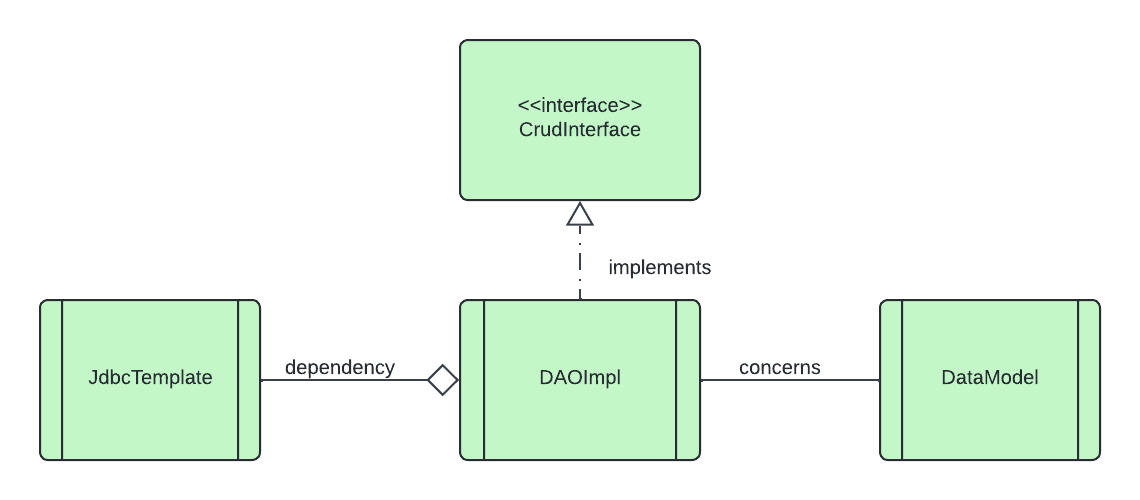
\includegraphics[width=0.8\linewidth]{images/jdbc_tem_businesslog.png}
    \end{framed}
    \caption{JDBC template}
    \label{fig:spring-logo}
\end{figure}

La mise en place de la couche de persistance dans ce contexte implique plusieurs étapes clés :

\begin{enumerate}
    \item \textbf{Configurer JdbcTemplate comme un Bean} : Dans une classe \textbf{\texttt{@Configuration}}, définissez \texttt{JdbcTemplate} comme un bean Spring. Cela permet à l'instance \texttt{JdbcTemplate} d'être injectée comme dépendance dans les classes DAO pour leur permettre d'effectuer des opérations sur la base de données.

    \item \textbf{Créer des modèles de données} : Définissez des classes de modèle de données qui représentent les entités dans la base de données. Ces classes seront utilisées pour mapper les enregistrements de la base de données aux objets Java.

    \item \textbf{Définir l'interface CRUD} : Créez une interface qui spécifie les opérations CRUD (Créer, Lire, Mettre à jour, Supprimer). Cette interface sera implémentée par les DAOs pour gérer l'accès aux données de manière cohérente.

    \item \textbf{Implémenter les DAOs} : Développez des classes DAO qui fournissent des implémentations concrètes des opérations CRUD définies dans l'interface. Ces classes utiliseront \texttt{JdbcTemplate} pour interagir avec la base de données.
\end{enumerate}

\begin{figure}[H]
    \centering
    \begin{framed}
        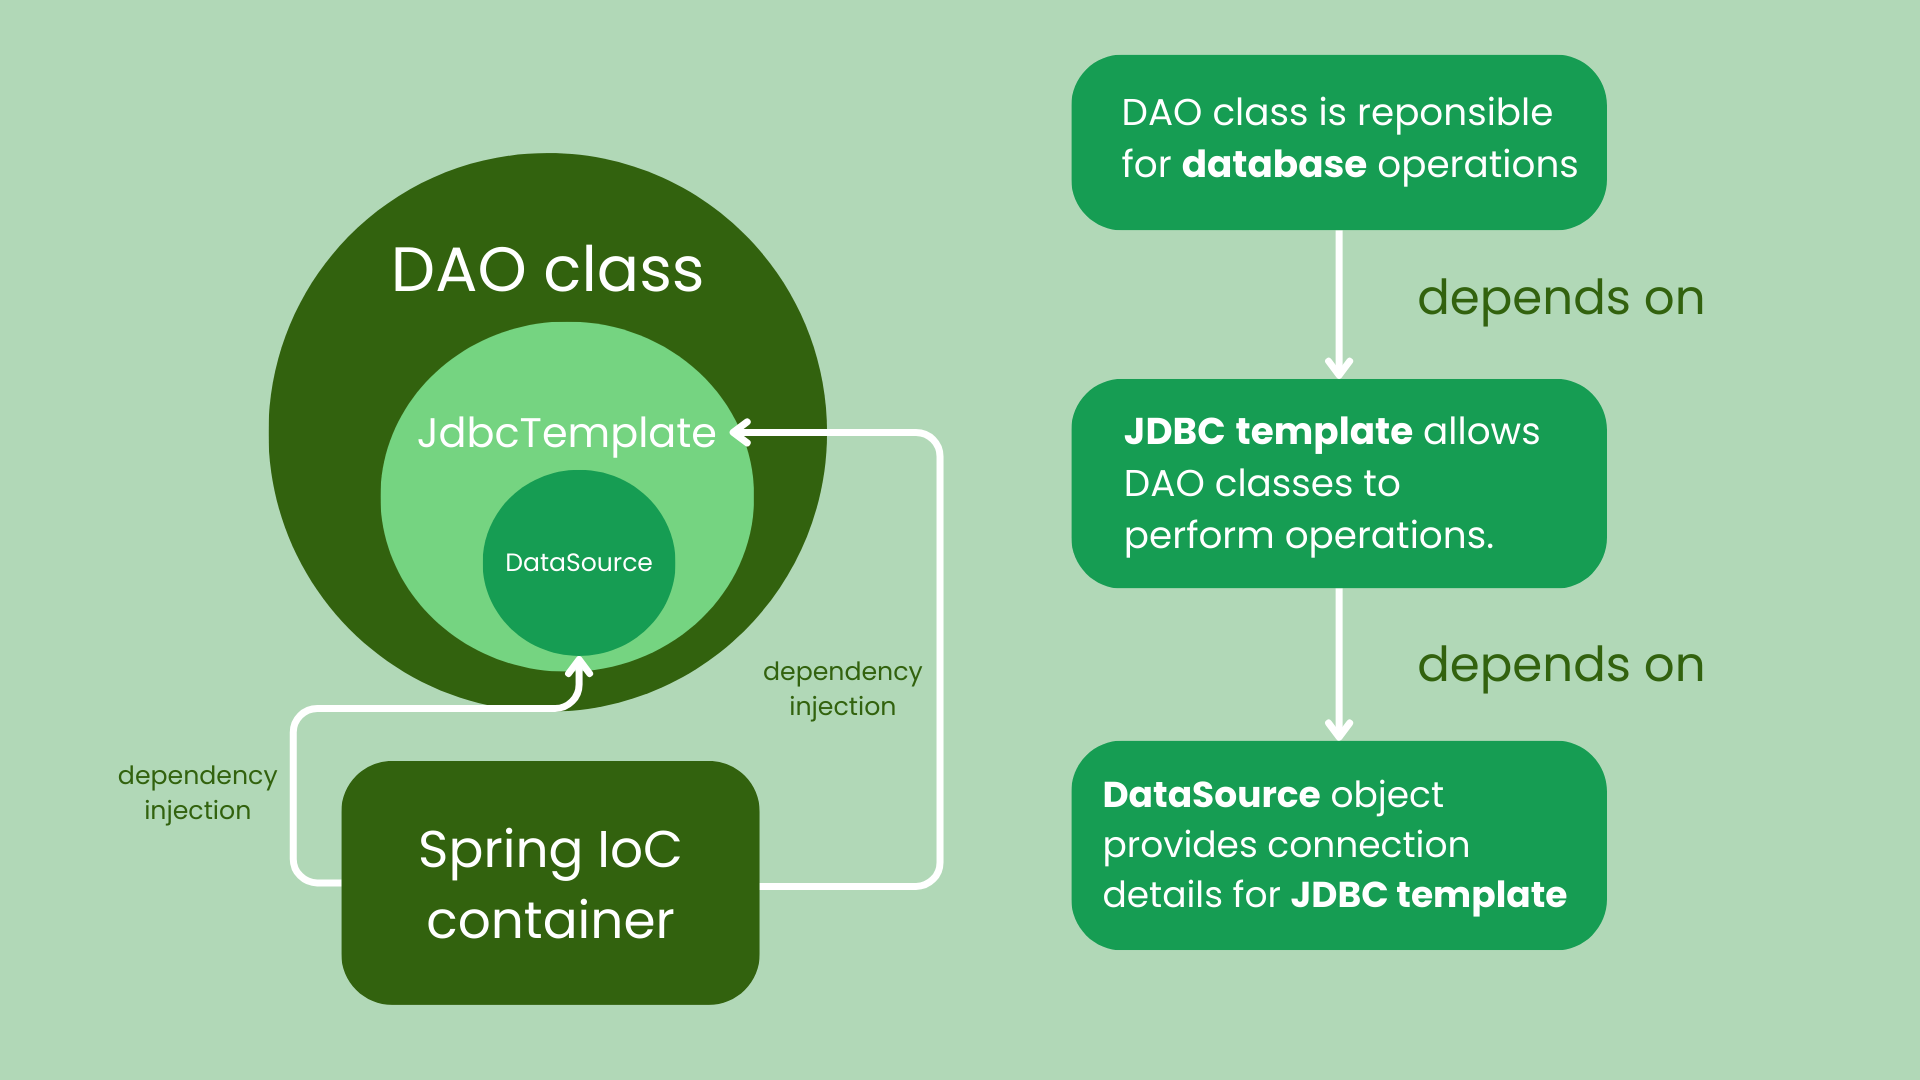
\includegraphics[width=0.8\linewidth]{images/minimalistic_jdbctemplate.png}
    \end{framed}
    \caption{Injection de dépendance dans la couche de persistance}
    \label{fig:spring-logo}
\end{figure}
\subsection{Exemple de code}

L'exemple suivant montre l'implémentation d'une couche de persistance pour la gestion d'une entité \texttt{Product} à l'aide de Spring JDBC. Il comprend la configuration de la base de données, un modèle de données, une interface DAO et une implémentation DAO. Le code complet est disponible sur le dépôt GitHub du projet : \\ \url{https://github.com/D0esN0tM1tter/spring_boot_project-/tree/master/supporting_project/persistence_examples/jdbctemplate_example}.

\subsubsection{Configuration de la base de données}

La classe \textbf{DatabaseConfig} définit le bean \texttt{JdbcTemplate}, qui est essentiel pour exécuter des opérations SQL dans les applications Spring.

\textbf{Explication :}
\begin{itemize}
    \item \texttt{JdbcTemplate} : Un utilitaire fourni par Spring pour interagir avec la base de données de manière simple et efficace.
    \item \texttt{DataSource} : Injecté dans le \texttt{JdbcTemplate}, il fournit la connexion à la base de données.
\end{itemize}

\subsubsection{Modèle de données Product}

La classe \textbf{Product} sert de modèle de données pour l'entité \texttt{Product}, représentant un enregistrement dans la base de données.

\textbf{Explication :}
\begin{itemize}
    \item Les annotations \texttt{@Data}, \texttt{@AllArgsConstructor} et \texttt{@NoArgsConstructor} de Lombok génèrent automatiquement le code standard comme les getters, setters et constructeurs.
    \item Les champs comme \texttt{id}, \texttt{label} et \texttt{price} sont directement liés aux colonnes de la table de la base de données.
\end{itemize}

\subsubsection{Interface DAO Product}

L'interface \textbf{ProductDao} définit les opérations CRUD pour l'entité \texttt{Product}.

\textbf{Explication :}
\begin{itemize}
    \item Des méthodes comme \texttt{save}, \texttt{update} et \texttt{deleteById} gèrent la logique de persistance pour l'entité \texttt{Product}.
    \item \texttt{findById} et \texttt{findAll} permettent de récupérer un ou plusieurs produits, respectivement.
\end{itemize}

\subsubsection{Implémentation DAO}

La classe \textbf{ProductDaoImpl} implémente l'interface \texttt{ProductDao}, fournissant des méthodes concrètes pour interagir avec la base de données.

\textbf{Explication :}
\begin{itemize}
    \item \texttt{RowMapper} : Permet de mapper chaque ligne du jeu de résultats à un objet \texttt{Product}.
    \item \texttt{KeyHolder} : Capture l'ID généré automatiquement lorsqu'un nouveau produit est inséré dans la base de données.
    \item Chaque méthode utilise \texttt{JdbcTemplate} pour exécuter les requêtes SQL de manière efficace.
\end{itemize}

\section{Approche Java Persistence API}

Cette section décrit l'utilisation de l'API Java Persistence (JPA) et Hibernate pour implémenter une couche de persistance dans les applications Java. Elle couvre une introduction à JPA, le processus de configuration pour établir une connexion à la base de données, ainsi que l'intégration de la logique métier.

\subsection{JPA et Hibernate}

L'API de persistance Java (JPA) est une spécification standard pour le mappage objet-relationnel (ORM) en Java. Elle offre une approche indépendante de la plate-forme pour interagir avec les bases de données relationnelles en mappant les objets Java sur des tables de base de données. Hibernate est une implémentation populaire de JPA qui propose des fonctionnalités ORM avancées et une intégration transparente avec JPA.

\textbf{Principales caractéristiques :}
\begin{itemize}
    \item Élimine le code redondant pour la gestion des opérations de base de données.
    \item Fournit des annotations pour mapper les classes Java aux tables de base de données.
    \item Offre un langage de requête (JPQL) pour interagir avec la base de données de manière orientée objet.
    \item Gère automatiquement les connexions et transactions de base de données.
\end{itemize}

\textbf{Avantages de JPA et Hibernate :}
\begin{itemize}
    \item Simplifie les opérations sur la base de données grâce à la gestion des entités.
    \item Réduit le risque d'injection SQL en utilisant des requêtes paramétrées.
    \item Améliore la portabilité entre différentes bases de données.
\end{itemize}

\subsection{Configuration de la connexion}

Pour utiliser JPA et Hibernate dans un projet, certaines configurations sont nécessaires pour établir une connexion à la base de données et gérer les entités. Dans une application Spring Boot, les paramètres de connexion et de JPA peuvent être configurés dans le fichier \texttt{application.properties}.

\textbf{Étapes pour la configuration :}
\begin{enumerate}
    \item Ajouter les dépendances pour JPA et Hibernate dans le fichier \texttt{pom.xml} (Maven) ou \texttt{build.gradle} (Gradle).
    \item Créer un fichier de configuration (\texttt{application.properties}) pour définir les propriétés de la base de données telles que l'URL, le nom d'utilisateur, le mot de passe et les paramètres spécifiques à Hibernate.
    \item Annoter les classes Java avec des annotations JPA (\texttt{@Entity}, \texttt{@Table}, etc.) pour les définir comme des entités mappées aux tables de la base de données.
    \item Utiliser \texttt{EntityManagerFactory} pour créer un \texttt{EntityManager}, qui fournit une interface pour interagir avec le contexte de persistance.
\end{enumerate}

\textbf{Configuration des propriétés de l'application :}
Pour configurer la connexion à la base de données MySQL dans une application Spring Boot, les propriétés suivantes doivent être ajoutées au fichier \texttt{application.properties} :

\textbf{Exemple de configuration de \texttt{application.properties} :}

\begin{lstlisting}[language=properties]
# Configuration de la base de données MySQL
spring.datasource.url=jdbc:mysql://localhost:3306/testdb?useSSL=false&serverTimezone=UTC
spring.datasource.username=root
spring.datasource.password=
spring.datasource.driver-class-name=com.mysql.cj.jdbc.Driver
spring.jpa.database-platform=org.hibernate.dialect.MySQL5InnoDBDialect
spring.jpa.hibernate.ddl-auto=update
spring.jpa.show-sql=true
spring.jpa.properties.hibernate.format_sql=true
\end{lstlisting}

Cette configuration garantit que Spring Boot utilise Hibernate comme fournisseur JPA et établit la connexion à la base de données MySQL avec les identifiants et paramètres nécessaires.

\subsection{Logique métier des données}

La couche de logique métier interagit avec la couche de persistance pour effectuer des opérations CRUD et appliquer des règles métier.

\textbf{Responsabilités de la couche logique métier :}
\begin{itemize}
    \item Valider et transformer les données avant la persistance.
    \item Coordonner entre la couche de persistance et les autres couches de l'application (par exemple, les contrôleurs).
    \item Gérer les transactions de base de données, garantissant la cohérence des données.
    \item Abstraire la logique de persistance de la couche de présentation.
\end{itemize}

\textbf{Utilisation des Repositories :}
Les repositories dans JPA sont des interfaces qui permettent de définir et de gérer les interactions avec la base de données avec un minimum de code standard. Hibernate peut étendre ces repositories pour fournir des requêtes personnalisées et des fonctionnalités avancées.

\textbf{Gestion du cycle de vie des entités :}
JPA fournit différents états pour les entités tels que \textit{transient}, \textit{persistent}, et \textit{detached}, permettant aux développeurs de gérer efficacement le cycle de vie des entités.

\subsection{Exemple de code}
Dans cette section, nous allons passer en revue un exemple simple montrant comment configurer et utiliser JPA avec Hibernate dans une application Spring Boot. Le code complet est disponible sur le dépôt GitHub du projet :\\ \url{https://github.com/D0esN0tM1tter/spring_boot_project-/tree/master/supporting_project/persistence_examples/jpa_examples}.
\vspace{0.5cm}\\
\textbf{Étape 1 : Classe d'entité}

Pour définir une entité JPA, nous devons annoter la classe avec \texttt{@Entity} et la mapper à une table dans la base de données en utilisant \texttt{@Table}. De plus, nous utilisons \texttt{@Id} pour marquer le champ clé primaire et \texttt{@GeneratedValue} pour la génération automatique de l'ID.

\textbf{Explication :}
\begin{itemize}
    \item \texttt{@Entity} : Marque la classe comme une entité JPA.
    \item \texttt{@Id} : Spécifie la clé primaire de l'entité.
    \item \texttt{@GeneratedValue} : Configure la stratégie de génération de la clé primaire (par exemple, \texttt{IDENTITY} pour les IDs auto-incrémentés).
    \item \texttt{@Column} : Mappe les champs aux colonnes de la base de données, avec des options comme \texttt{nullable} pour définir les contraintes des colonnes.
\end{itemize}

\subsubsection{Repository du Produit}

L'interface du repository étend \texttt{JpaRepository}, offrant des opérations CRUD intégrées.

\textbf{Explication :}
\begin{itemize}
    \item \texttt{JpaRepository} : Fournit des méthodes telles que \texttt{save()}, \texttt{findById()}, \texttt{findAll()} et \texttt{deleteById()} pour les opérations de base de données sans avoir besoin de mises en œuvre personnalisées.
    \item Des méthodes de requête personnalisées peuvent être ajoutées si nécessaire.
\end{itemize}

\subsubsection{Couche Service}

La couche service interagit avec le repository pour gérer la logique métier.

\textbf{Explication :}
\begin{itemize}
    \item La couche service est utilisée pour abstraire la logique métier, rendant la couche contrôleur plus claire.
    \item L'annotation \texttt{@Autowired} injecte le repository, permettant une injection de dépendances facile.
    \item Les méthodes telles que \texttt{saveProduct()} et \texttt{getProductById()} offrent un accès aux méthodes du repository pour créer, récupérer et supprimer des produits.
\end{itemize}

\subsubsection{Couche Contrôleur}

Le contrôleur expose les méthodes du service via des points de terminaison RESTful pour l'interaction avec le front-end.

\textbf{Explication :}
\begin{itemize}
    \item \texttt{@RestController} : Marque la classe comme un contrôleur REST qui gère les requêtes HTTP.
    \item \texttt{@RequestMapping} : Spécifie l'URL de base pour les points de terminaison du contrôleur.
    \item \texttt{@PostMapping}, \texttt{@GetMapping} et \texttt{@DeleteMapping} : Gèrent respectivement les requêtes HTTP POST, GET et DELETE.
    \item \texttt{@RequestBody} et \texttt{@PathVariable} : Gèrent les charges utiles des requêtes et les paramètres d'URL dynamiques.
\end{itemize}

\textbf{Étape 5 : Configuration de l'application}

Assurez-vous que l'application est correctement configurée pour exécuter une application Spring Boot avec JPA. Les détails de la configuration peuvent être définis dans le fichier \texttt{application.properties}, comme décrit dans la section précédente.

Cette configuration crée un flux complet pour gérer les entités dans une application Spring Boot avec JPA et Hibernate. Avec une configuration minimale, Spring Boot gère la plupart du code redondant, permettant aux développeurs de se concentrer sur la logique métier.

\section{Conclusion}

Dans ce chapitre, nous avons exploré différentes approches pour gérer la couche de persistance dans une application Spring Boot. Nous avons couvert l'implémentation de la persistance avec JDBC, détaillant la configuration de la base de données, les modèles de données et les interfaces CRUD, ainsi que l'utilisation de \texttt{JdbcTemplate} pour interagir avec la base de données. En parallèle, nous avons également abordé la configuration de la persistance avec JPA et Hibernate, la configuration de la connexion à la base de données et la définition des entités à l'aide des annotations JPA. Ces deux approches offrent des avantages différents en fonction des besoins du projet : JDBC pour des opérations plus manuelles et contrôlées, et JPA/Hibernate pour une gestion automatisée et un mappage objet-relationnel simplifié. En combinant ces techniques, nous pouvons construire une couche de persistance robuste, flexible et maintenable.

\end{document}
